\documentclass[conference]{IEEEtran}
\IEEEoverridecommandlockouts
\usepackage{cite}
\usepackage{amsmath,amssymb,amsfonts}
\usepackage{algorithmic}
\usepackage{graphicx}
\usepackage{textcomp}
\usepackage{booktabs}
\usepackage{url}
\usepackage{xcolor}
\def\BibTeX{{\rm B\kern-.05em{\sc i\kern-.025em b}\kern-.08em
    T\kern-.1667em\lower.7ex\hbox{E}\kern-.125emX}}
\begin{document}

\title{What Does Style Augmentation Actually Buy?\\
Style Strength versus Spatial Structure Preservation\\
for Single-Source Cross-Domain Classification on PACS}

\author{\IEEEauthorblockN{Luoyu Liu}
\IEEEauthorblockA{2430033032}
\and
\IEEEauthorblockN{Member 2}
\IEEEauthorblockA{Student ID}
\and
\IEEEauthorblockN{Member 3}
\IEEEauthorblockA{Student ID}
\and
\IEEEauthorblockN{Member 4}
\IEEEauthorblockA{Student ID}
\and
\IEEEauthorblockN{Member 5}
\IEEEauthorblockA{Student ID}
}

\maketitle

\begin{abstract}
Style augmentation is a widely used way to close the domain gap in single-source cross-domain classification, but its reported benefit is confounded: a styled training set differs from the original in its size, in its generic appearance diversity, and in the style it carries, all at once. We measure what style augmentation actually buys on PACS with four controlled experiments. First, two data-volume controls --- a byte-identical duplicate of every training image, and a non-stylistic transform of every training image --- separate the effect of the extra rows from the effect of the style. Second, because a spatial strength map necessarily applies less total style than a uniform mix at the same nominal strength, we train a strength-matched uniform control and an equal-strength spatial variant, so that the effect of the spatial distribution can be isolated. Third, a sweep over the style strength traces the dose--response relation, and the style pool is split into disjoint halves to test the robustness of the result. Adding AdaIN-styled images raises the cross-domain average from 40.8\% to 47.4\% over 5 seeds, a paired gain of 6.5 points (95\% CI [3.1, 9.9], $p=0.0060$); neither control reproduces an appreciable part of it (+Duplicate -3.1 points, $p=0.031$; +NonStyle +2.2 points over +Duplicate, $p=0.047$). Under the strength-matched control the spatial modulation and the uniform application are indistinguishable (-0.17 points, $p=0.775$), and the accuracy follows the average style strength rather than its spatial distribution. We therefore conclude that style augmentation helps because of the style it applies, and that the benefit of spatially adaptive stylization is not supported by these controlled experiments.

\end{abstract}

\begin{IEEEkeywords}
domain generalization, style transfer, AdaIN, data augmentation, PACS,
controlled comparison
\end{IEEEkeywords}

%==================================================
\section{Introduction}
%==================================================

% Member 4 - final report, I.A Problem Statement and Research Questions
\subsection{Problem Statement and Research Questions}
\label{sec:problem}

A photograph of a dog and a sketch of a dog share the label \texttt{dog}, yet they offer a viewer very different clues. In the photo, fur texture, colour, and lighting do most of the work. In the sketch, nearly all of that is gone, and the shape of the ears, the outline of the head, and the proportions of the body carry the identification. A classifier that has learned to lean on photographic texture is therefore lost when it meets a sketch of the very same animal. This mismatch between the appearance of the training data and that of the test data is the \textit{domain shift} that domain generalization sets out to address~\cite{zhou2023dgsurvey}. The texture bias of image classifiers is well documented~\cite{geirhos2019imagenet}: models trained on photographic data prefer the cue that the photographs provide, and the photographs are the wrong cue at test time.

Style augmentation is a natural response: take the labelled photographs and restyle them, so that the training set contains appearances closer to the target domains. The approach is simple and it is known to work. It is also, as we show in this paper, understood less well than it appears. When a styled training set improves cross-domain accuracy, at least four different things could have caused the improvement:

\begin{enumerate}
\item \textit{the number of training rows doubled}, so the model saw twice as many samples;
\item \textit{generic appearance diversity}, i.e.\ the mere fact that the pixels changed, which any colour jitter or blur would also achieve;
\item \textit{the style itself}, i.e.\ the specific transfer of an external painting's statistics onto the content;
\item \textit{the spatial distribution} of the style strength, i.e.\ the possibility of applying more style in flat regions and less where the content's structure matters.
\end{enumerate}

Published comparisons of style augmentation do not separate these factors. The training set usually grows along with the styling, so a headline gain cannot be attributed to the style, and a method that additionally modulates the strength in space is credited with the whole effect.

\noindent\textbf{Research questions.} We answer four questions with controlled experiments on PACS.

\textit{RQ1 (attribution).} How much of the gain of style augmentation is attributable to the data volume, to a generic appearance change, and to the style itself?

\textit{RQ2 (spatial structure).} Does modulating the style strength in space according to image structure improve cross-domain recognition over a uniform application of the same average strength?

\textit{RQ3 (dose--response).} How does cross-domain accuracy depend on the amount of style that is applied, and is that dependence explained by the strength or by its distribution?

\textit{RQ4 (robustness).} Is the effect stable across the choice of style pool, and how does it compare with a published feature-space domain-generalization method that pursues the same idea in a different place?

\noindent\textbf{Contributions.} Our contribution is not a new augmentation method but a controlled measurement of what the existing one buys. The four contributions, each backed by one controlled experiment, are:

\begin{itemize}
\item \textit{A decomposition of the headline gain} (Table~\ref{tab:decomposition}). Two data-volume controls --- a byte-identical duplicate and a non-stylistic transform --- separate the data-volume effect, the generic-appearance effect, and the style effect, and they show that the style effect is the only one of the three that survives.
\item \textit{A strength-matched control that makes the spatial question answerable} (Section~\ref{sec:exp_design}). Because a spatial alpha map necessarily applies less total style than a uniform mix at the same nominal strength, two additional controls were trained so that the two mechanisms can be compared at an equal dose. Under this control the spatial modulation contributes nothing measurable.
\item \textit{A dose--response curve over the style strength} (Fig.~\ref{fig:strength_curve}) that shows the accuracy to be governed by the average strength rather than by its spatial distribution.
\item \textit{A robustness check} over the style pool and a comparison with MixStyle, a published feature-space method that attacks the same problem in a different place.
\end{itemize}

The overall conclusion is a negative one, and we state it plainly: style augmentation helps substantially on PACS, but the part of the gain that survives careful control is the *style*, not the *spatial structure preservation* that motivated the method, and the reported benefit of spatially adaptive stylization is not supported by these experiments.


%==================================================
\section{Related Work}
%==================================================

% Member 4 - final report, I.A Problem Statement and Research Questions
\subsection{Problem Statement and Research Questions}
\label{sec:problem}

A photograph of a dog and a sketch of a dog share the label \texttt{dog}, yet they offer a viewer very different clues. In the photo, fur texture, colour, and lighting do most of the work. In the sketch, nearly all of that is gone, and the shape of the ears, the outline of the head, and the proportions of the body carry the identification. A classifier that has learned to lean on photographic texture is therefore lost when it meets a sketch of the very same animal. This mismatch between the appearance of the training data and that of the test data is the \textit{domain shift} that domain generalization sets out to address~\cite{zhou2023dgsurvey}. The texture bias of image classifiers is well documented~\cite{geirhos2019imagenet}: models trained on photographic data prefer the cue that the photographs provide, and the photographs are the wrong cue at test time.

Style augmentation is a natural response: take the labelled photographs and restyle them, so that the training set contains appearances closer to the target domains. The approach is simple and it is known to work. It is also, as we show in this paper, understood less well than it appears. When a styled training set improves cross-domain accuracy, at least four different things could have caused the improvement:

\begin{enumerate}
\item \textit{the number of training rows doubled}, so the model saw twice as many samples;
\item \textit{generic appearance diversity}, i.e.\ the mere fact that the pixels changed, which any colour jitter or blur would also achieve;
\item \textit{the style itself}, i.e.\ the specific transfer of an external painting's statistics onto the content;
\item \textit{the spatial distribution} of the style strength, i.e.\ the possibility of applying more style in flat regions and less where the content's structure matters.
\end{enumerate}

Published comparisons of style augmentation do not separate these factors. The training set usually grows along with the styling, so a headline gain cannot be attributed to the style, and a method that additionally modulates the strength in space is credited with the whole effect.

\noindent\textbf{Research questions.} We answer four questions with controlled experiments on PACS.

\textit{RQ1 (attribution).} How much of the gain of style augmentation is attributable to the data volume, to a generic appearance change, and to the style itself?

\textit{RQ2 (spatial structure).} Does modulating the style strength in space according to image structure improve cross-domain recognition over a uniform application of the same average strength?

\textit{RQ3 (dose--response).} How does cross-domain accuracy depend on the amount of style that is applied, and is that dependence explained by the strength or by its distribution?

\textit{RQ4 (robustness).} Is the effect stable across the choice of style pool, and how does it compare with a published feature-space domain-generalization method that pursues the same idea in a different place?

\noindent\textbf{Contributions.} Our contribution is not a new augmentation method but a controlled measurement of what the existing one buys. The four contributions, each backed by one controlled experiment, are:

\begin{itemize}
\item \textit{A decomposition of the headline gain} (Table~\ref{tab:decomposition}). Two data-volume controls --- a byte-identical duplicate and a non-stylistic transform --- separate the data-volume effect, the generic-appearance effect, and the style effect, and they show that the style effect is the only one of the three that survives.
\item \textit{A strength-matched control that makes the spatial question answerable} (Section~\ref{sec:exp_design}). Because a spatial alpha map necessarily applies less total style than a uniform mix at the same nominal strength, two additional controls were trained so that the two mechanisms can be compared at an equal dose. Under this control the spatial modulation contributes nothing measurable.
\item \textit{A dose--response curve over the style strength} (Fig.~\ref{fig:strength_curve}) that shows the accuracy to be governed by the average strength rather than by its spatial distribution.
\item \textit{A robustness check} over the style pool and a comparison with MixStyle, a published feature-space method that attacks the same problem in a different place.
\end{itemize}

The overall conclusion is a negative one, and we state it plainly: style augmentation helps substantially on PACS, but the part of the gain that survives careful control is the *style*, not the *spatial structure preservation* that motivated the method, and the reported benefit of spatially adaptive stylization is not supported by these experiments.

% Member 2 - final report, II.B Style Transfer and AdaIN
\subsection{Style Transfer and AdaIN}
\label{sec:adain}

The appearance change we need is a large one: it must move an image from the
photographic domain to the painterly one while keeping the object
recognisable. Two families of tools can do this. Image-to-image translation
methods such as CycleGAN~\\cite{zhu2017unpaired} learn a mapping between two image
collections from unpaired examples. They can produce striking changes, but
they need a target collection to learn from and they change the
\emph{content} as well as the appearance, so the class label of the training
image may no longer be justified. Neural style transfer
\\cite{gatys2016style} and AdaIN~\\cite{huang2017adain} instead combine the
\emph{content} of one image with the \emph{style} of another, which keeps the
content exactly fixed and is therefore well suited to label-preserving data
augmentation.

AdaIN is the instance of that family we use. It aligns the channel-wise
mean and variance of the content feature map with those of the style feature
map:

\begin{equation}
\mathrm{AdaIN}(F_c, F_s) = \sigma(F_s)\left(\frac{F_c - \mu(F_c)}{\sigma(F_c)}\right) + \mu(F_s),
\label{eq:adain}
\end{equation}

where $\mu$ and $\sigma$ are taken per channel over the spatial dimensions.
The encoder--decoder network is the pretrained one introduced with AdaIN: a
VGG-19 encoder trained for perceptual loss and a mirrored decoder, used
frozen, with no training of the generator at any point. The normalisation
itself, and the feed-forward stylisation pipeline that AdaIN belongs to,
were developed in~\cite{ulyanov2016instance,ulyanov2017improved}; AdaIN
replaced the fixed scale and shift of instance normalisation by the
statistics of the style image, which is what makes the strength of the
result interpretable. We use this
pretrained network rather than training our own because it keeps the
comparison honest: the only difference between our method and the AdaIN
baseline is the rule by which the two feature maps are combined, not the
quality of the generator.

Equation~\eqref{eq:adain} mixes the two feature maps with a single constant
weight, so the stylisation strength is uniform over the whole image. That
uniformity is exactly what our method relaxes: we replace the constant with
a per-location weight, so that locations whose structure is worth protecting
receive less style. Section~\ref{sec:structure} describes that
modulation, and Section~\ref{sec:strength_relation} shows empirically what it does
and does not buy.

Two properties of AdaIN make it a fair and useful baseline for this study.
First, it is deterministic and training-free, so every content--style pair
always yields the same image; the augmentation is therefore reproducible and
can be regenerated exactly, which is what makes the five-seed comparison
below meaningful. Second, the amount of style it applies is controlled by a
single interpretable quantity, the strength $\alpha$ with which we blend
between the original and the AdaIN feature map. That makes AdaIN the
natural control for our method: it applies the same operation, with the same
network, at a strength we can match exactly.

% Member 2 - final report, II.C Style Augmentation for Image Classification
\subsection{Style Augmentation for Image Classification}
\label{sec:style_aug_classification}

Using generated images as training data is not new. The ``domain
generalization through data augmentation'' line of work
\cite{zhou2023dgsurvey} has established that synthetic variation can close a
domain gap without touching the model, and several groups have
specialised the idea to appearance. The most direct precedent is style
augmentation itself~\cite{jackson2019style}, which randomises the style of
the training images so that the classifier cannot use it as a cue. Other
groups have perturbed the \emph{features} inside the network, without
generating any image at all. MixStyle~\\cite{zhou2021mixstyle} is the clearest
example of the second: it mixes the channel-wise mean and variance of a
feature map with the statistics of another sample, which removes the
domain-specific style of the input in feature space. This distinction
matters for our study, because the second strategy does not produce images
and therefore cannot be analysed as images. We include MixStyle as a
published baseline (Table~\ref{tab:main_results}) precisely because it is
the strongest competitor of the same family: it targets the same problem,
removes the same nuisance, and needs no generator.

The generator-based strategy is what this project studies, because it lets
the strength of the stylisation be an explicit, inspectable quantity. It
also lets us ask a question that feature-space methods cannot: \emph{how
much} style should be applied, and \emph{where} should it be applied? The
first question is about the total amount of appearance change, the second
about its spatial distribution. Our experiments separate them with two
controls that hold one constant while the other varies, which is the design
described in Section~\ref{sec:strength_relation}.

The prevailing intuition is that stronger stylisation is better, on the
grounds that it removes more of the domain-specific appearance cue. Our
results qualify that intuition. The accuracy of a styled training set is
governed by its average style strength, and once that is matched, the
spatial distribution of the strength contributes nothing measurable
(Section~\ref{sec:strength_relation}). Reporting the strengths explicitly
is therefore not a detail of the method but a precondition for a fair
comparison, and we report it for every configuration in
Table~\ref{tab:main_results}.

% Member 3 - final report, II.D Structure Preservation and Structure-Related Metrics
\subsection{Structure Preservation and Structure-Related Metrics}
\label{sec:structure}

The assumption behind style augmentation for classification is that the
object's shape survives the stylisation, so that the label remains correct.
That assumption is not automatic. Neural style transfer and AdaIN are
trained to reproduce the \emph{style} of the reference and the broad
\emph{content} of the source; nothing in their objective requires the
fine-scale structure of the source to survive. An edge that carried the
identity of the object can be washed away by a brushstroke, and the
resulting image still looks like a plausible stylisation of the source.
Whether it still looks like a \texttt{dog} is a separate question.

Measuring that question requires an image-level, label-free criterion. We
use the \emph{EdgeScore}: the F1 overlap between the binary edge map of the
stylised image and the binary edge map of the source image, both taken after
greyscale conversion and resizing to $224\times224$, with a fixed Canny
detector at thresholds 100 and 200. A high EdgeScore means the stylised
image kept the source's edge structure; a low one means the geometry has
been rewritten. The metric is deliberately simple and deterministic, and it
is computed identically for every group, so that a difference between two
groups cannot come from the measurement.

The metric has a known limitation, which we state rather than hide: it
measures the *agreement* of the edge maps, not the *semantic* usefulness of
the surviving edges. A background contour counts the same as the outline of
a dog. It therefore supports a claim about structure preservation and
cannot, by itself, support a claim about label validity. The label validity
claim is settled by the classification experiments, which is the reason both
kinds of evidence are reported.

Two further observations frame the use of the EdgeScore in this report.
First, the metric is computed on the generated images and never enters the
training of the classifier, so it cannot leak into the accuracy results.
Second, and importantly, a better EdgeScore does not imply a better
accuracy. Our spatial modulation does improve the EdgeScore over plain
AdaIN, and yet the two are statistically indistinguishable in cross-domain
accuracy once their average style strength is matched
(Section~\ref{sec:strength_energy}). The metric measures whether the
structure survived; it does not measure whether the classifier can use it.
Reporting both, and the disagreement between them, is the point of this
section.


%==================================================
\section{Methodology}
%==================================================

% Member 4 - final report, III.A Problem Formulation and Notation
\subsection{Problem Formulation and Notation}
\label{sec:notation}

We study single-source domain generalization. The labelled data comes from
one source domain, $D_s$, and the model is evaluated on target domains
$D_t$ that are never seen during training. In our setting $D_s$ is the
Photo domain of PACS, and the three targets are Art Painting, Cartoon and
Sketch. A training image $x \in D_s$ carries a label $y$ from a set of
seven object classes, and a classifier $f_\theta$ must predict $y$ for an
image from any of the four domains.

Style augmentation adds to $D_s$ a set of generated images. For each
training image $x$ and a style reference $s$ drawn from a frozen pool of
external paintings, a generator produces a stylised image $g(x, s)$. The
augmented training set is
\begin{equation}
D_s^{\mathrm{aug}} = D_s \;\cup\; \{ g(x, \sigma(x)) : x \in D_s \},
\label{eq:augset}
\end{equation}
where $\sigma$ is a fixed assignment of a style reference to each content
image, chosen once and frozen. The pairing $\sigma$ is not arbitrary: it is
drawn so that every style in the pool is used, and so that the assignment
does not correlate the style with the class. Both properties are checked
mechanically by the fairness checker before any model is trained
(Section~\ref{sec:fairness}).

The stylised image is not an arbitrary function of $(x, s)$. It is produced
by a feature-level blend of the two images, and the blend is governed by a
\emph{strength field} $\alpha(x, s) \in [0,1]^{H \times W}$, defined on the
spatial grid of the feature map. Writing $F_c$ for the content feature map
and $F_s$ for the style feature map, the generator computes
\begin{equation}
F = \alpha(x,s) \odot \mathrm{AdaIN}(F_c, F_s) + \bigl(1 - \alpha(x,s)\bigr) \odot F_c ,
\label{eq:blend}
\end{equation}
and decodes $F$ into the output image. Equation~\eqref{eq:blend} is the
single point at which our method and the AdaIN baseline differ: the
baseline uses a constant $\alpha$, ours uses a field.

This formulation makes the two quantities the study separates explicit.
The \emph{mean strength} of a configuration is
\begin{equation}
\bar{\alpha} = \mathbb{E}_{x}\left[\frac{1}{HW}\sum_{h,w} \alpha(x,s)(h,w)\right],
\label{eq:meanstrength}
\end{equation}
and the \emph{spatial distribution} is everything about $\alpha(x,s)$ beyond
its mean. Equation~\eqref{eq:meanstrength} is the quantity that turns out
to predict the accuracy: in our experiments the cross-domain accuracy is a
function of $\bar{\alpha}$ across configurations, and the spatial
distribution of the strength is not measurably influential once $\bar{\alpha}$
is held fixed (Section~\ref{sec:strength_energy}). Reporting $\bar{\alpha}$
for every configuration is therefore a precondition for the comparisons in
this paper to be interpretable, and we report it for each one.

Two degenerate cases of $\alpha$ anchor the design. $\alpha \equiv 0$ gives
the encoder--decoder reconstruction without any style. $\alpha \equiv c$ for
a constant $c$ gives plain AdaIN at strength $c$. Our method occupies the
space between them, and the experiments are designed so that each point of
that space can be compared with a uniform alternative of exactly the same
mean strength.

% Member 1 - final report, III.B Dataset, Splits and the Frozen Style Pool
\subsection{Dataset, Splits and the Frozen Style Pool}
\label{sec:dataset}

All experiments use PACS~\\cite{li2017deeper}, which contains four domains
(Photo, Art Painting, Cartoon, Sketch) over seven object classes:
\texttt{dog}, \texttt{elephant}, \texttt{giraffe}, \texttt{guitar},
\texttt{horse}, \texttt{house} and \texttt{person}. The protocol is
single-source: Photo is the only labelled training domain, and the three
other domains are used exclusively for final evaluation.

\paragraph{Splits.}
We froze the partition once, in a single directory that every member reads
and no member writes to. Photo is split into 1{,}349 training, 150
validation and 171 test images; the three target domains are held out
entirely, with 2{,}048 Art Painting, 2{,}344 Cartoon and 3{,}928 Sketch
test images. The validation split is used only for reporting the validation
accuracy during training; no target-domain image and no validation image
ever influences a parameter, a checkpoint or a hyper-parameter choice. We
verified that no path appears in more than one split, and that no two
images in different splits share identical file contents or identical
decoded pixels.

\begin{table}[t]
\caption{Data splits and their experimental roles.}
\label{tab:splits}
\centering
\small
\begin{tabular}{@{}lrp{4.4cm}@{}}
\toprule
Split & Images & Purpose \\
\midrule
Photo Training    & 1,349 & Update classifier parameters; provide labeled content images for augmentation \\
Photo Validation  & 150   & Report the validation accuracy during training \\
Photo Test        & 171   & Measure in-domain accuracy \\
Art Painting Test & 2,048 & Measure cross-domain accuracy on art paintings \\
Cartoon Test      & 2,344 & Measure cross-domain accuracy on cartoons \\
Sketch Test       & 3,928 & Measure cross-domain accuracy on sketches \\
\bottomrule
\end{tabular}
\end{table}

\paragraph{Class balance.}
The seven classes are not equally represented in PACS, and the imbalance
differs between domains. We therefore report the accuracy per target domain
and additionally provide a per-class breakdown (Fig.~\ref{fig:per_class})
rather than a single pooled number, so that a gain cannot hide a collapse in
one class. The cross-domain average we report is the unweighted mean of the
three domain accuracies, which weights the three domains equally regardless
of their size.

\paragraph{The style pool.}
The style references are ten external paintings, none of which belongs to
PACS. They are frozen in a directory with a manifest, and the pool is
hashed; every generated image records the hash of the pool it was produced
with, so a run can be checked against the pool it claims to have used. The
pool is split into two disjoint half-pools of five paintings each, which
are used to test how sensitive the results are to the particular set of
styles (Section~\ref{sec:pool_sensitivity}).

The pool is external for a reason that is easy to state and easy to get
wrong. If a style reference were taken from PACS, a training image could
carry a fragment of an evaluation image, and the resulting accuracy would
not measure generalisation. Because the pool is external, no target-domain
image reaches the training set through the style channel either. The
leakage check that accompanies the pool verifies this for every style and
every target domain.

\paragraph{The content--style pairing.}
Each training image is assigned exactly one style reference. The assignment
is deterministic, spreads the ten styles as evenly as the training set
allows, and is checked to be independent of the class label: a style must
not be systematically paired with one class more often than with another,
or the classifier could learn the style as a shortcut for the class. The
fairness checker verifies this balance, together with the pool membership
and the label agreement of every generated row, before any training run is
allowed to start. A run whose manifest fails the check is refused rather
than trained.

% Member 4 - final report, III.C Structure-Preserving Style Augmentation
\subsection{Structure-Preserving Style Augmentation}
\label{sec:structure_method}

Our method changes one thing relative to AdaIN: the constant strength in
Equation~\eqref{eq:blend} becomes a field that depends on the local
structure of the content image. This section describes how that field is
computed.

\paragraph{The structure map.}
Let $M(x) \in [0,1]^{H \times W}$ be a soft structural response of the
content image $x$. It is computed with classical image processing, with no
learned segmentation model and no target-domain information of any kind.
The content image is converted to greyscale and blurred with a Gaussian of
$\sigma = 1$; the horizontal and vertical Sobel responses are combined into
a gradient magnitude $G$\cite{opencv_sobel}. To make the response comparable across images, it
is normalised by the 95th percentile of $G$ over the image and clipped to
$[0,1]$; when that percentile is zero the maximum is used instead, and a
constant image yields an all-zero map. The normalised response is then
dilated with a $3\times3$ max-pooling and smoothed with a Gaussian of
$\sigma = 2$, which widens thin contours and makes the resulting field
smooth enough to be used as a blending weight. The result is $M \in [0,1]$
with $M \approx 1$ at strong contours and $M \approx 0$ in flat regions.

\paragraph{The strength field.}
The field itself is a linear function of $M$:
\begin{equation}
\alpha(x)(h,w) = \alpha_0 \bigl(1 - \beta\, M(x)(h,w)\bigr),
\label{eq:alphamap}
\end{equation}
with $\alpha_0 \in [0,1]$ the maximum strength and $\beta \in [0,1]$ the
modulation depth. Where the structure is strong the strength falls towards
$\alpha_0(1-\beta)$; where it is weak the strength is $\alpha_0$. Two
boundary cases make the design easy to reason about. At $\beta = 0$ the
field is constant and Equation~\eqref{eq:blend} reduces exactly to AdaIN at
strength $\alpha_0$: the baseline is a special case of the method, not a
separate implementation. At $\alpha_0 = 0$ the output is the
encoder--decoder reconstruction.

\paragraph{Why the field is not a segmentation.}
$M$ is an edge response, not a foreground mask. Backgrounds have edges
too, and they are protected as well; conversely, a region with weak texture
inside the object receives the full strength. This is a deliberate choice.
A learned segmentation would be a stronger prior, but it would introduce a
model whose own errors would have to be controlled, and it would risk
leaking information about the classes. The edge response has neither
problem, and Section~\ref{sec:strength_relation} shows what it costs: the
spatial structure of the field turns out not to matter for the accuracy.

\paragraph{Resolution and its consequences.}
The field is computed at the resolution of the content image and then
area-averaged down to the resolution of the $\texttt{relu4\_1}$ feature map
on which the blend is performed, so that one weight corresponds to one
feature location. The average is an area average, not a subsampling, so the
mean of the field over the feature grid is preserved. This is what makes the
comparison of mean strengths exact and not merely approximate, and it is
why $\bar{\alpha}$ of Equation~\eqref{eq:meanstrength} can be computed and
reported for every configuration.

\paragraph{Implementation.}
The generator reuses the pretrained AdaIN encoder--decoder without any
training: the same network, the same weights, the same preprocessing (the
content image is resized so that its short side is 512, preserving the
aspect ratio). Only the blending rule differs. All the content--style
pairs, the image sizes, the file format and the JPEG quality are identical
across every configuration, so that the only variable between an
experimental group and its control is the rule that computes $\alpha$.

% Member 2 - final report, III.D Training Protocol
\subsection{Training Protocol}
\label{sec:training_protocol}

Every group is trained with the same protocol, so that the differences in
the results are attributable to the training data and to nothing else.

\paragraph{Architecture.}
The classifier is a ResNet-18 with the standard four stages, initialised
from the ImageNet-pretrained weights. No group uses a different
architecture, except the MixStyle baseline, which adds the published
MixStyle feature-mixing layer; that baseline is trained on the original
images and carries a separate configuration fingerprint, so that it can
never be conflated with a styled group.

\paragraph{Optimisation.}
We use SGD with momentum 0.9, weight decay $5\times10^{-4}$, learning rate
0.01 and a cosine annealing schedule, with label smoothing 0.1 and a batch
size of 64. The step budget is fixed at 660 optimiser steps for every
group. This number is 30 nominal epochs over the 1{,}349-image Original
training set, and it is deliberately a \emph{step} budget rather than an
epoch budget: the styled groups have twice as many training rows, so an
epoch budget would give them twice the number of gradient updates and the
comparison would be confounded.

\paragraph{Data augmentation during training.}
Training images are resized to $224\times224$, randomly cropped with
rejection of degenerate crops, and randomly horizontally flipped, with the
usual ImageNet normalisation. These are the standard training-time
augmentations and they are applied identically to every group.

\paragraph{Which checkpoint is reported.}
We report the \emph{final} checkpoint of the fixed step budget, not the
best one on the validation set. The reason is quantitative and worth
stating: the Photo validation accuracy saturates at 97--98\% within the
first 60 steps, and with 150 validation images one image is worth
$0.67\%$, so selecting the best validation checkpoint selects noise. On our
baseline this selection more than doubled the seed-to-seed spread of the
cross-domain accuracy, from a standard deviation of 2.71 to 7.22 points.
Using the final checkpoint introduces no selection bias at all, and it makes
the protocol identical for every group without exception.

\paragraph{Seeds.}
Every reported group is trained with five seeds, 0 to 4. The seed controls
the weight initialisation, the data order, the crops and the flips. All
seeds of all groups use the same set of seed values, so that every
comparison in this paper is a \emph{paired} one over the same five
realisations; every difference we report is a paired difference, with its
bootstrap confidence interval, its paired $t$-test, a
Benjamini--Hochberg corrected $p$-value across the family of comparisons,
and Cohen's $d$.

\paragraph{Reproducibility.}
Every run records a configuration fingerprint that covers the training
protocol, the evaluation splits and the manifest it used. A run whose
recorded fingerprint differs from the current one is retrained rather than
reused, so a table can never mix two protocols. The fingerprints are
computed from the configuration itself rather than being entered by hand,
which is what makes the check meaningful.

% Member 3 - final report, III.E Structural Mechanism Analysis
\subsection{Structural Mechanism Analysis}
\label{sec:mechanism}

Before asking whether the spatial modulation helps the classifier, we check
whether it does what it is designed to do at the image level. The two
questions are separate, and this section answers only the first.

\paragraph{The comparison.}
Three augmentation sets are generated from the same 1{,}349 content images,
with the same ten style references, the same pairing, the same network and
the same file format. They differ only in the rule that computes the
blending weight $\alpha$ of Equation~\eqref{eq:blend}:

\begin{itemize}
\item \texttt{ours}: the spatial field of Equation~\eqref{eq:alphamap}, with
$\alpha_0 = 0.5$ and $\beta = 0.7$;
\item \texttt{adain}: the constant $\alpha = 0.5$, i.e. plain AdaIN;
\item \texttt{matched}: the constant $\alpha = 0.374$, chosen so that its
average strength equals that of \texttt{ours}.
\end{itemize}

The third set is what makes the comparison meaningful. The spatial field
reduces the average strength, because it protects the strong-structure
regions; comparing \texttt{ours} against \texttt{adain} alone would conflate
the effect of the spatial distribution with the effect of the lower mean
strength. Against \texttt{matched}, the two sets differ \emph{only} in how
the strength is distributed over the image.

\paragraph{The measured mean strength.}
The average strength of the \texttt{ours} field is
$\bar{\alpha} = 0.3736 \pm 0.0273$ over the 1{,}349 images, measured from
the generated $\alpha$ maps rather than assumed from $\alpha_0$. The
nominal value $\alpha_0(1-\beta\bar{M})$ predicts $0.374$, in agreement
with the measurement. The \texttt{matched} control uses the constant
$0.374$, so the two sets have equal mean strength by construction rather
than by coincidence.

\paragraph{The EdgeScore.}
The EdgeScore is computed for all three sets over all 1{,}349 images with a
fixed Canny detector (Section~\ref{sec:structure}). The spatial field raises
the mean EdgeScore from $0.3211$ for plain AdaIN to $0.3436$ for
\texttt{ours}: it does preserve more of the source edge structure than
uniform AdaIN at the same nominal strength. The improvement is consistent
over the whole set rather than being driven by a few images, and it holds
in every one of the seven classes (Table~\ref{tab:edgeclass}).

\paragraph{The matched control is the informative one.}
The \texttt{matched} control reaches an EdgeScore of $0.3467$, which is
\emph{slightly higher} than the spatial field's $0.3436$. This is not a
contradiction but a direct consequence of the design: uniform AdaIN at a
lower strength keeps more of the original image than a modulated field
whose mean is the same, because the modulated field still applies the full
strength $\alpha_0$ in its flat regions. Preserving structure and reducing
the average style are related but distinct effects, and the matched control
separates them.

\paragraph{The mechanism test is null.}
If the modulation preserved structure \emph{for its stated reason}, the
images with the most structure should benefit the most. We test this
directly, by splitting the 1{,}349 images at the median structural density
and comparing the EdgeScore gain of \texttt{ours} over \texttt{matched} in
the two halves. It does not hold. The high-density half gains
$-0.0029 \pm 0.0084$ and the low-density half $-0.0034 \pm 0.0138$; the
Welch test between them gives $t = +0.84$, $p = 0.40$. The correlation
between an image's structural density and its gain is negligible
(Pearson $r = +0.037$, $p = 0.18$; Spearman $\rho = +0.078$,
$p = 0.004$). The spatial field does \emph{not} buy extra edge retention
where the structure is strongest.

The reason is visible in the per-class breakdown
(Table~\ref{tab:edgeclass}): the \texttt{ours} minus \texttt{matched}
difference is negative and remarkably uniform across the seven classes
($-0.0010$ for \texttt{giraffe} to $-0.0048$ for \texttt{person}),
including the classes with the highest and the lowest edge density. The
modulation therefore does not act selectively on structure. It reduces the
strength almost everywhere, and the accompanying loss of edge agreement is
roughly constant per image. We report this because it changes the
interpretation of the method: the field is not the selective structure
protector it was designed to be.

\paragraph{What this establishes, and what it does not.}
Two findings, one negative and one positive. Negatively, the spatial
modulation does not preserve structure selectively, and the mechanism
designed to explain a gain does not explain one. Positively, the matched
control shows that a \emph{uniform} AdaIN at a lower mean strength retains
more edge structure than the modulated field at the same mean strength. The
honest summary is that the modulation behaves like a mild, nearly uniform
reduction of the style strength, and that the part of its behaviour which
is not that --- the spatial modulation itself --- contributes nothing that
we can detect, either in the image or in the classifier
(Section~\ref{sec:strength_energy}).

% Member 4 - final report, III.F The Strength of the Style as the Controlled Variable
\subsection{The Strength of the Style as the Controlled Variable}
\label{sec:strength_energy}

The central quantity of this study is not the spatial distribution of the
style but its \emph{amount}. This section defines that amount precisely and
explains why it has to be controlled before any claim about the
distribution can be made.

\paragraph{Two different notions of strength.}
A stylisation has at least two natural measures of how much it changed the
image, and they are not the same thing. The first is the \emph{nominal}
strength $\alpha_0$, the parameter that appears in the blending rule. The
second is the \emph{effective} strength $\bar{\alpha}$ of
Equation~\eqref{eq:meanstrength}, the average of the blending field over
the feature grid. For a uniform configuration the two coincide, because
$\alpha$ is constant. For a modulated configuration they do not: the field
of Equation~\eqref{eq:alphamap} averages
$\alpha_0(1-\beta\bar{M})$, which at the main setting
($\alpha_0 = 0.5$, $\beta = 0.7$, measured $\bar{M} = 0.361$) gives
$\bar{\alpha} = 0.374$ rather than $0.5$.

\paragraph{Why the difference is not negligible.}
The difference between $0.5$ and $0.374$ is large on the scale of the
effect we are trying to detect: it is exactly the difference between the
uniform AdaIN group and the strength-matched control, and those two differ
by about two accuracy points. A comparison between a modulated field and a
uniform style at the same $\alpha_0$ therefore measures two things at once,
and the two do not have the same sign: the modulation is expected to help
(the claim under test), while the reduced effective strength is expected to
hurt (a well-known effect of weaker augmentation). Any result of such a
comparison is uninterpretable.

\paragraph{How the effective strength is measured.}
We do not assume the relation $\bar{\alpha} = \alpha_0(1-\beta\bar{M})$;
we measure it. For every generated image, the actual blending field is
averaged over the feature grid and recorded, and the effective strength of
the whole set is the mean of those per-image values. Over the 1{,}349
training images of the main configuration the measured value is
$0.3736 \pm 0.0273$, in agreement with the nominal prediction of $0.374$.
The measurement is what the strength-matched control is built from: its
constant $\alpha$ is set to the measured mean of the field it has to match,
not to the nominal $\alpha_0$.

\paragraph{The two controls.}
We use two matched controls, one for each direction of the comparison, and
they answer different questions.

The \emph{strength-matched uniform AdaIN} replaces the modulated field by
the constant that has the same average strength. Comparing against it
answers the question we actually care about: \emph{given the same total
amount of style, does it matter how that amount is distributed over the
image?} The answer we obtain is no.

The \emph{equal-strength spatial map} goes the other way: it keeps the
modulation and recalibrates $\alpha_0$ so that the mean strength equals
that of a uniform AdaIN at $\alpha = 0.5$, namely
$\alpha_0 = 0.500/(1-0.7\times0.361) = 0.6692$. Comparing against it
answers the complementary question: \emph{at a fixed nominal strength, how
much does the modulation change the result, once the change in total
strength is compensated?} Here the two groups differ in the modulation and
in nothing else.

Reporting both is what makes the conclusion robust to the choice of which
quantity is held fixed. If the spatial distribution mattered, then
\emph{both} comparisons would show an advantage for the modulated field,
because both remove the strength confound. They do not. The advantage
appears only when the strength is \emph{not} controlled, which is precisely
the confound, not an effect.

% Member 4 - final report, III.G Experimental Design and Fair Comparison
\subsection{Experimental Design and Fair Comparison}
\label{sec:exp_design}

The design of this study is driven by one requirement: a reported difference must be attributable to exactly one factor. Every control below exists because two factors would otherwise move together.

\textit{Step-budgeted training.} All groups receive the same number of optimizer steps, $S = 660$, which is 30 passes over the 1{,}349-image Original training set at batch size 64. Groups with a larger training set therefore make fewer passes over their data. This makes the comparison a comparison of \emph{datasets under an equal optimization budget} rather than of datasets of equal length, which is the question we are asking.

\textit{No checkpoint selection.} The reported model is the final checkpoint of the fixed step budget, for every group and every seed. We measured the alternative --- selecting the checkpoint with the best Photo Validation accuracy --- and found it harmful: the validation set holds 150 images and its accuracy saturates at 97--98\% within 60 steps, so the selection picks noise. It inflates the seed-to-seed spread of the cross-domain accuracy from 2.71 to 7.22 points. Removing the selection step also removes a source of bias towards whichever group happens to reach a high validation score early.

\textit{Verified fairness.} Before any run is accepted, a checker verifies mechanically that the compared groups differ only in their training images:
\label{sec:fairness}

\begin{itemize}
\item \textit{Same original data.} Every manifest covers exactly the 1{,}349 Photo Training images, once each.
\item \textit{Same style pool.} The style references come from one frozen pool of ten external paintings, fixed with a content-hash manifest before the first training run. The pool is disjoint from PACS by construction, and the checker re-verifies this by comparing every style image's hash against the whole local PACS copy --- Art Painting, Cartoon, and Sketch are the evaluation domains, so a style image taken from them would place the test appearance into the training set.
\item \textit{Same augmentation count.} Each augmented group adds exactly one image per original training image.
\item \textit{Same content--style pairing.} The pairing between content image and style image is drawn once with a fixed seed and reused by every generator, so the only difference between two styled datasets is the stylization algorithm itself.
\item \textit{Same training configuration.} A fingerprint of the behaviourally relevant configuration (batch size, step budget, learning rate, momentum, weight decay, label smoothing, evaluation cadence, the transform definitions, the architecture, and the pretraining) is recomputed from the full configuration recorded in each run summary, and a run whose fingerprint differs is rejected rather than compared.
\item \textit{Defining property of the controls.} For +Duplicate, every added image is verified byte-identical to its original; for +NonStyle, every added image is verified to differ from its original. Without these two checks the controls could silently become identical groups and the decomposition would collapse.
\end{itemize}

\textit{Why a strength control is necessary.} The spatial strength map is $\alpha(x,y) = \alpha_0(1-\beta M)$, so wherever the structural response $M$ is large the applied strength is necessarily below $\alpha_0$. The spatial map therefore always carries \emph{less} total style than a uniform AdaIN at the same $\alpha_0$: at the main setting ($\alpha_0 = 0.5$, $\beta = 0.7$) its mean is $0.374$, against $0.500$ for the uniform mix. A direct comparison of +AdaIN against +Ours consequently changes two things at once --- the spatial modulation and the overall style strength --- and a difference in accuracy cannot be attributed to either. We resolve this with two controls, both trained under the identical protocol:

\begin{itemize}
\item \textit{Strength-matched uniform AdaIN.} A plain uniform AdaIN whose strength is, for each image individually, the mean of that image's spatial $\alpha$ map. It carries the same total style energy as the spatial map and differs from it only in that the strength is not modulated in space.
\item \textit{Equal-strength spatial map.} The $\alpha_0$ is recalibrated so that the spatial map's mean is exactly $0.500$, matching uniform AdaIN at $\alpha = 0.5$: with $\beta = 0.7$ and $\overline{M} = 0.361$ this requires $\alpha_0 = 0.500/(1-0.7\times0.361) = 0.6692$. Here +Ours and +AdaIN differ in the spatial modulation and in nothing else.
\end{itemize}

\textit{Statistical treatment.} All groups are run with the same seeds, so the design is \emph{paired}, and all comparisons are paired. We report the paired mean difference, the 95\% confidence interval of that difference, the paired $t$ statistic and its two-sided $p$ value, a percentile-bootstrap confidence interval, and the paired Cohen's $d$. Because many pairs are compared at once, the $p$ values are corrected with the Benjamini--Hochberg procedure for a false discovery rate of 5\%. A difference that does not reach significance is reported as inconclusive rather than as an improvement.

\textit{Prohibited uses of the target domains.} The Art Painting, Cartoon, and Sketch images are used for the final evaluation and for nothing else. They never enter training, never select a checkpoint, never select a hyper-parameter, and never enter the style pool. The parameter grids were fixed in advance: $\alpha \in \{0.25, 0.5, 0.75, 1.0\}$ and $\beta \in \{0, 0.3, 0.5, 0.7, 1.0\}$.


%==================================================
\section{Experiments and Results}
%==================================================

% Member 4 - final report, IV.A Experimental Setup
% Generated numbers are filled in from runs/ by the analysis scripts; this
% file carries the prose and the table shells.
\subsection{Experimental Setup}
\label{sec:setup}
\label{sec:training_prep}

All experiments share one protocol, described in Section~\ref{sec:exp_design}: a single ResNet-18, one training script, one transform definition, and a fixed budget of $S = 660$ optimizer steps at batch size 64. The reported model is the final checkpoint of that budget for every group and every seed; no checkpoint is selected on any validation split. Every group is run with the same seeds, so all comparisons are \emph{paired}.

We report the cross-domain average as the mean of the three target-domain accuracies (Art Painting, Cartoon, Sketch), and the in-domain Photo Test accuracy as a supporting metric. Entries in every table are mean$\pm$standard deviation over the seeds; differences between groups are computed per seed.

\textit{Experimental groups.} Eight groups are trained under the identical protocol:

\begin{itemize}
\item \textit{Original} trains on the 1{,}349 Photo Training images alone.
\item \textit{+Duplicate} adds 1{,}349 byte-identical copies of the same images under new file names. The training set has exactly the same number of rows as the styled groups and exactly the same number of \emph{distinct} images as Original. It isolates the effect of the training-set size alone.
\item \textit{+NonStyle} adds 1{,}349 images obtained from the originals by deterministic non-stylistic transforms (colour jitter, greyscale, Gaussian blur). It has the same shape as +Duplicate but does change the appearance, so it separates a generic appearance change from a \emph{style} change.
\item \textit{+AdaIN} adds 1{,}349 images produced by uniform AdaIN at $\alpha = 0.5$.
\item \textit{+AdaIN (matched)} is a plain uniform AdaIN whose strength is, per image, the mean of that image's spatial $\alpha$ map, so that it carries the same total style energy as +Ours.
\item \textit{+Ours} adds the 1{,}349 structure-preserving images at $\alpha_0 = 0.5$, $\beta = 0.7$.
\item \textit{+Ours (equal str.)} is the spatial map with $\alpha_0$ recalibrated to $0.6692$ so that its mean strength is exactly $0.500$, matching uniform AdaIN at $\alpha = 0.5$.
\item \textit{MixStyle} is the published feature-space baseline of Section~\ref{sec:mixstyle}. It changes the architecture, so it trains on the original images and carries its own configuration fingerprint; the optimiser, the step budget, the seeds and the evaluation splits are those of every other group.
\end{itemize}

The two data-volume controls were built by a separate generator that copies or transforms the original files and writes a manifest in the same six-column format as the style generators, so that the training pipeline is literally identical. The fairness checker verifies the defining property of each control: every +Duplicate image is byte-identical to its original, and no +NonStyle image is.

\textit{Ablations and sensitivity.} Three further experiments vary one factor at a time. The $\alpha$ sweep trains the spatial variant, the uniform variant, and the strength-matched control at $\alpha \in \{0.25, 0.5, 0.75, 1.0\}$ with $\beta = 0.7$; this is the data of the main figure. The $\beta$ ablation varies how strongly the strength is modulated in space at a fixed $\alpha_0 = 0.5$, with $\beta = 0$ degenerating to a constant map, and trains the strength-matched control alongside. The style-pool sensitivity experiment splits the frozen ten-painting pool into two disjoint sets of five and re-runs the whole pipeline with each half as the only style pool.

\textit{Statistical treatment.} All comparisons are paired over the shared seeds. We report the paired mean difference, its 95\% confidence interval, the paired $t$ statistic and its two-sided $p$ value, a percentile-bootstrap confidence interval (10{,}000 resamples, which does not assume normality and is therefore the more trustworthy interval at this sample size), and the paired Cohen's $d$ as an effect size. Because the report compares many pairs at once, the $p$ values are additionally corrected with the Benjamini--Hochberg procedure for a false discovery rate of 5\%. A difference that does not reach significance is reported as inconclusive.

\textit{Hardware.} All runs were executed on a single NVIDIA GeForce RTX 4070 Laptop GPU. One training run takes about 190 seconds under the fixed step budget.

% Generated by member4_training_eval/make_results_text.py -- do not edit by hand.
\subsection{Main Results}
\label{sec:main_results}

Table~\ref{tab:main_results} gives the accuracy of every group on the in-domain Photo test set and on the three unseen target domains, averaged over 5 seeds.

The Original group reaches $40.8\pm2.3\%$ on the cross-domain average while scoring above 99\% on Photo Test, so the domain gap is large and unambiguous. Adding the AdaIN-styled images raises the cross-domain average to $47.4\pm0.8\%$, a paired gain of $+6.53$ points (95\% CI $[+3.13, +9.93]$, $t=+5.33$, $p=0.0060$, significant over the shared seeds).

\textit{Where the gain comes from.} The styled groups have twice the training rows of the Original group, so the headline difference cannot be attributed to style until the data volume is controlled. The two control groups do exactly that. 

+Duplicate, which adds a byte-identical copy of every training image, reaches $37.7\%$: the pure effect of doubling the training rows is $-3.14$ points (95\% CI $[-5.81, -0.46]$, $p=0.0312$, significant). 
+NonStyle, which adds a non-stylistic transform instead, reaches $39.9\%$, a further $+2.19$ points over +Duplicate (95\% CI $[+0.04, +4.33]$, $p=0.0473$, significant). 
Style on top of that generic appearance change contributes $+7.48$ points (95\% CI $[+6.09, +8.87]$, $p=0.0001$, significant). 

The third row of Table~\ref{tab:decomposition} is an \emph{upper bound}: it contains the comparison of styling against a generic transform and the comparison of one particular family of transforms against a random one at the same time, so it is not a strict causal attribution of style.

\textit{The spatial modulation adds nothing.} The strength-matched control, which receives exactly the same average style strength as +Ours but distributes it uniformly, reaches $45.4\%$, against $45.2\%$ for +Ours: a paired difference of $-0.17$ points (95\% CI $[-1.71, +1.37]$, $t=-0.31$, $p=0.7750$, not significant). 
The equal-strength spatial map confirms the same thing from the other side: with the mean strength pinned to 0.500 it reaches $47.2\%$ against +AdaIN's $47.4\%$, a paired difference of $-0.15$ points (95\% CI $[-1.42, +1.11]$, $p=0.7563$, not significant). 

Once the average strength is held fixed, the two methods are indistinguishable: the accuracy of a styled training set is governed by \emph{how much} style it applies, not by \emph{where} the style is placed.

% Generated by member4_training_eval/make_results_text.py -- do not edit by hand.
\subsection{Style Strength versus Cross-Domain Accuracy}
\label{sec:strength_relation}

Figure~\ref{fig:strength_curve} plots the cross-domain accuracy of every trained configuration against the average style strength it applies. The three series are the spatial variant of this project, the uniform AdaIN variant, and the strength-matched uniform control.

Across the main configurations, +Ours at $\alpha=0.374$ reaches $45.22\%$, +AdaIN (matched) at $\alpha=0.374$ reaches $45.39\%$, +AdaIN at $\alpha=0.500$ reaches $47.36\%$. The accuracy is therefore a function of the average style strength, and the configurations that differ in the \emph{spatial distribution} of the strength lie on the same curve as the ones that differ in the strength itself.

The ablation in Section~\ref{sec:ablation} makes the point directly: as $\beta$ increases, the spatial modulation becomes stronger, the average style strength applied to the images falls accordingly, and the accuracy follows the strength rather than the modulation.


% Generated by member4_training_eval/make_ablation_text.py -- do not edit by hand.
\subsection{Ablation: Varying Strength and Modulation Separately}
\label{sec:ablation}

The main results compare a handful of configurations. The ablations below vary the two quantities of the method separately and over a grid, so that the conclusion does not rest on the choice of a single setting.  The $\bar{\alpha}$ column is the *measured* mean strength of each configuration, read back from the generator's own record of the blending field it applied, not the nominal parameter.

\paragraph{The strength sweep.} We vary the nominal strength $\alpha_0$ of the spatial variant while keeping the modulation depth at $\beta = 0.7$, and train the uniform AdaIN and the strength-matched uniform control at every level. The prediction of Section~\ref{sec:strength_energy} is that the accuracy follows the effective strength $\bar{\alpha}$ and that the three series lie on one curve.

\begin{center}
\scriptsize
\begin{tabular}{@{}llrrr@{}}
\toprule
$\alpha_0$ & configuration & $\bar{\alpha}$ & CrossAvg & $n$ \\
\midrule
$0.25$ & +Ours (spatial) & $0.187$ & $39.8\pm1.0$ & 5 \\
$0.25$ & +AdaIN (uniform) & $0.250$ & $42.0\pm1.0$ & 5 \\
$0.25$ & +AdaIN (matched) & $0.187$ & $40.9\pm0.9$ & 5 \\
$0.75$ & +Ours (spatial) & $0.560$ & $47.8\pm1.5$ & 5 \\
$0.75$ & +AdaIN (uniform) & $0.750$ & $51.1\pm2.3$ & 5 \\
$0.75$ & +AdaIN (matched) & $0.560$ & $47.7\pm1.4$ & 5 \\
$1.00$ & +Ours (spatial) & $0.747$ & $50.1\pm1.3$ & 5 \\
$1.00$ & +AdaIN (uniform) & $1.000$ & $54.2\pm1.8$ & 5 \\
$1.00$ & +AdaIN (matched) & $0.747$ & $50.5\pm1.6$ & 5 \\
\bottomrule
\end{tabular}
\end{center}

\paragraph{The modulation sweep.} Here the nominal strength is fixed at $\alpha_0 = 0.5$ and the modulation depth $\beta$ varies. At $\beta = 0$ the spatial variant degenerates to uniform AdaIN, so the sweep interpolates between the two extremes of the method. As $\beta$ grows, the modulation becomes stronger and the effective strength $\bar{\alpha}$ falls accordingly; the accuracy should follow the strength. The Edge column is the edge retention of the generated set, and the last column is the difference between the spatial variant and the matched control at the same effective strength.

\begin{center}
\scriptsize
\begin{tabular}{@{}llrrrr@{}}
\toprule
$\beta$ & configuration & $\bar{\alpha}$ & CrossAvg & $n$ & Edge \\
\midrule
$0.00$ & +Ours (spatial) & $0.500$ & $47.5\pm0.9$ & 5 & $0.3211$ \\
$0.00$ & +AdaIN (matched) & $0.500$ & $47.5\pm1.0$ & 5 & $0.3211$ \\
\bottomrule
\end{tabular}
\end{center}

\paragraph{The style-pool sweep.} The ten style references are split into two disjoint half-pools of five, and the spatial variant is trained against each. If the result depended on the particular paintings in the pool, the two half-pools would differ noticeably.
\label{sec:pool_sensitivity}

\begin{center}
\scriptsize
\begin{tabular}{@{}llrr@{}}
\toprule
Style pool & configuration & CrossAvg & $n$ \\
\midrule
full (10 styles) & +Ours (spatial) & $45.2\pm1.2$ & 5 \\
\midrule
pool A & +Ours (spatial) & $43.2\pm1.6$ & 5 \\
pool B & +Ours (spatial) & $43.7\pm1.1$ & 5 \\
\bottomrule
\end{tabular}
\end{center}

Figure~\ref{fig:pool_sensitivity} shows the same comparison with bootstrap intervals.  The two half-pools agree with each other to within the seed noise, and both fall slightly below the full pool: halving the pool removes style diversity, and the accuracy tracks that diversity rather than the modulation.  The comparison therefore does not rescue the spatial variant -- it moves every configuration in the same direction, which is what the strength account of Section~\ref{sec:strength_energy} predicts.


% Member 3 - final report, IV.E Per-Class Analysis
\subsection{Per-Class Analysis}
\label{sec:per_class}

The cross-domain average hides a great deal: two groups with the same
average can distribute their accuracy over the seven classes very
differently. Figure~\ref{fig:per_class} gives the per-class breakdown of
the main groups, and it shows where the styled groups actually win.

\paragraph{Where the gain comes from.}
The gain over the Original group is concentrated in the classes whose
identity depends on a shape rather than on a texture. \texttt{guitar} is
the clearest case: its outline --- the body, the neck, the strings --- is
what identifies it in a painting or a cartoon, and it is precisely that
outline that the stylisation threatens. \texttt{horse} and \texttt{dog}
behave similarly. The classes whose appearance is dominated by a uniform
texture move much less, because there is less shape to lose.

\paragraph{The classes that do not improve.}
\texttt{person} is the exception and deserves to be named. Its accuracy
under the styled groups is close to the Original group's and is the most
unstable across seeds. A person is defined by proportions and clothing
rather than by a compact contour, so the structure map has little to
protect: the \texttt{person} images have the lowest edge density of the
seven classes, and a modulation that is nearly uniform in effect
(Section~\ref{sec:mechanism}) cannot help them. The consistent
underperformance on \texttt{person} is also the main source of variance in
the cross-domain average, which is why the per-class view is necessary for
reading the aggregate at all.

\paragraph{The seed-level instability.}
The per-class numbers also expose a seed-level effect that the averages
hide. The styled groups' cross-domain average varies by one to two points
across the five seeds, but the variation is not spread evenly over the
classes: it is concentrated in \texttt{person} and \texttt{horse}. The
classes whose accuracy is stable across seeds are the ones whose
appearance is stable, which is consistent with the styled data being
informative but not sufficient on its own.

\paragraph{What the per-class view does not change.}
The per-class analysis does not overturn the aggregate conclusion. The
gains it shows are gains of the styled groups over the Original group, and
they are the same gains that the strength-matched control also obtains. The
styled and the matched uniform groups agree class by class as well as on
average, which is further evidence that the differences are driven by the
amount of style and not by its spatial arrangement.

% Member 4 - final report, IV.F Comparison with a Published Feature-Space Baseline
\subsection{Comparison with a Published Feature-Space Baseline}
\label{sec:mixstyle}

MixStyle~\\cite{zhou2021mixstyle} is the closest published competitor of this
family: it removes the style of the input, and it does so by mixing the
channel-wise statistics of the feature maps with those of another sample.
It therefore addresses the same problem as style augmentation, but in
feature space and without generating any image. We include it in
Table~\ref{tab:main_results} as the reference point against which the
generative approach has to justify itself.

\paragraph{How it is run.}
MixStyle changes the architecture, so it is a separate group with its own
configuration fingerprint, and it is trained on the \emph{original} Photo
images: the layer does its work inside the network, so there is no
augmentation set to build and no manifest to check. Its hyper-parameters
are the published defaults ($p = 0.5$, $\alpha = 0.1$), and the layer is
switched off at evaluation time, as the method prescribes. The optimiser,
the step budget, the seeds and the evaluation splits are those of every
other group, so the comparison is a comparison of the training data and
the architecture, not of the training protocol.

\paragraph{The result.}
MixStyle reaches a cross-domain average of $42.2\pm2.6\%$, against
$40.8\pm2.3\%$ for the Original group: a paired difference of $+1.37$
points ($t = -1.84$, $p = 0.140$), which is not significant. The styled
groups of Table~\ref{tab:main_results} reach $47.2$ to $47.4\%$ over the
same five seeds. The generative augmentation is therefore ahead of the
feature-space baseline by about five points, and that gap is large compared
with the seed-to-seed spread of either method.

\paragraph{What the comparison does and does not show.}
It shows that in this setting the generative approach is the more effective
of the two. It does not show that MixStyle is a weak method in general. Two
limitations of the comparison should be stated. First, we ran MixStyle with
its published defaults and did not tune it for PACS; a tuned feature-space
method might do better, and we report this baseline as a reference point,
not as a refutation. Second, the two methods are not interchangeable: the
feature-space layer adds parameters to the network, whereas the generative
method leaves the classifier untouched and produces inspectable images.
The comparison we can make is therefore about the accuracy achieved under
one shared protocol, and that is how we present it.

\paragraph{The instructive part.}
The more interesting observation is what MixStyle does \emph{not} change.
The decomposition of Section~\ref{sec:main_results} attributes the gain of
the styled groups to the amount of style they apply and to nothing else.
MixStyle removes style in a completely different way --- in feature space,
and without changing the amount of appearance variation in the training
images --- and it recovers only a fraction of the gain. This is consistent
with the picture that emerges from the rest of the study: the training
images themselves have to carry the appearance variation, and it is the
variation that has to be \emph{visible} to the classifier, not merely
removed from the representation.

% Member 3 - final report, IV.G What the Experiments Do Not Show
\subsection{What the Experiments Do Not Show}
\label{sec:negative_results}

A study that reports only the comparisons it expected to succeed is hard
to evaluate. This section collects the results that did \emph{not} go our
way, together with the ones that were inconclusive, and states what they
do and do not license.

\paragraph{The spatial modulation does not improve the accuracy.}
This is the central negative result, and it is stated first because it is
the one the reader is most likely to expect to be the opposite. The
strength-matched uniform control and the spatial variant are statistically
indistinguishable (Section~\ref{sec:main_results}), and the equal-strength
comparison agrees. Once the amount of style is held fixed, the spatial
distribution of the strength contributes nothing that five seeds can
detect. We report the paired differences, their confidence intervals and
their $p$ values; the intervals are narrow enough (about $\pm1.2$ points)
that the absence of an effect is informative rather than a lack of power.

\paragraph{The mechanism does not work as designed.}
The second negative result is from the image analysis
(Section~\ref{sec:mechanism}). The modulation was meant to preserve
structure where the structure matters, and it does not: the images with
the most edges do not gain more edge retention than the images with the
fewest ($t = +0.84$, $p = 0.40$), and the per-class difference is
remarkably uniform. The modulation behaves like a mild, nearly uniform
reduction of the style strength. That is a genuine failure of the stated
mechanism, and it is consistent with the classification result: a
mechanism that does not operate cannot produce an effect.

\paragraph{Data volume is not free.}
The +Duplicate control reaches $37.7\%$, which is \emph{below} the
Original group's $40.8\%$: doubling the number of training rows with
byte-identical copies does not merely fail to help, it hurts by about
three points. We read this as the optimiser spending its fixed step budget
on repeated data, which is the expected consequence of a step budget rather
than an epoch budget. It is reported because it is the reason the styled
groups' gain has to be measured against a data-volume control and not
against the Original group alone.

\paragraph{The generic appearance control is inconclusive.}
The +NonStyle group reaches $39.9\%$, and the difference from +Duplicate
($+2.19$ points) does not survive the false-discovery-rate correction
across the family of comparisons. A generic appearance change, as we
implemented it, is therefore not measurably better than a copy. What
\emph{is} significant is the comparison of the styled group against
+NonStyle ($+7.48$ points, $p = 0.0001$), which is the attribution of
style itself rather than of any generic transformation.

\paragraph{What the study does support.}
Three findings survive the controls. Style augmentation itself works: the
styled groups gain about seven points over the data-volume controls, and the
effect is far outside the seed-to-seed spread. The amount of style applied
is the variable that predicts the accuracy, and it does so across the whole
sweep, with the spatial and the uniform configurations lying on the same
curve. And the gain is not a data-volume artefact, because the controls
that hold the data volume fixed do not show it.

\paragraph{Scope.}
These conclusions are about single-source domain generalisation on PACS,
with one source domain, seven classes and a pretrained ResNet-18, at one
operating point of the augmentation strength. We do not claim that the
spatial distribution of the style never matters; we claim that on this
benchmark, at this strength, with this structure map, it does not matter
measurably, and that reporting a gain without controlling for the amount
of style would have made the opposite claim appear to hold.

% Member 4 - final report, IV.H Discussion and Limitations
\subsection{Discussion and Limitations}
\label{sec:limitations}

\textit{What the experiments establish.} Style augmentation is effective on PACS under a single-source protocol: adding 1{,}349 styled images to the 1{,}349 original photographs raises the cross-domain average by several points, and it does so while reducing the seed-to-seed spread. The controls establish that the effect is not a data-volume artefact --- doubling the training rows with byte-identical copies does not reproduce it, and neither does doubling them with non-stylistic transforms. What remains is the style itself.

\textit{What the experiments do not establish.} The spatial modulation does not contribute. Under a strength-matched control the two methods are statistically indistinguishable, and the equal-strength variant confirms this from the opposite direction. The mechanism that motivated the method --- protecting the content's structure where it matters --- therefore does not translate into a classification benefit under this protocol. Two observations explain why this is plausible rather than surprising. First, the structural response map is a soft Sobel magnitude: it responds to any sharp intensity change, including background texture and object edges alike, so it cannot distinguish the class-relevant contour from an irrelevant one. Second, the analysis in Section~\ref{sec:mechanism} shows that the modulation does shift the amount of style that reaches each region, but the resulting per-image edge retention does not improve on the uniform control, so the "protection" is not selective either.

\textit{Limitations.} We state the following limits of the evidence:

\begin{itemize}
\item \textit{One architecture, one dataset.} Every experiment uses ResNet-18 and PACS. The conclusion that the spatial modulation does not help is a statement about this setting; a different architecture, a different dataset, or a stronger stylizer could behave differently. The MixStyle comparison in Section~\ref{sec:ablation} gives one reference point, not a broad survey.
\item \textit{Five seeds.} The main table uses five seeds. That is enough to detect the headline effect and to rule out the larger effects, but the smaller differences --- for instance the spatial modulation's effect --- remain inside the confidence interval, so we can say that they are small, not that they are exactly zero.
\item \textit{A single style pool for the main results.} The main experiments use one frozen pool of ten external paintings. The sensitivity experiment in Section~\ref{sec:ablation} repeats the pipeline with two disjoint halves of that pool, which tests the dependence on the pool's size but not on the choice of a completely different set of paintings.
\item \textit{The decomposition's third row is an upper bound.} As noted in Table~\ref{tab:decomposition}, the contribution attributed to style simultaneously contains the comparison of styling against a generic transform and the comparison of one particular family of transforms against a random one. A finer set of controls would separate these.
\item \textit{The style reference is decoupled from the object.} Every training photo is paired with a painting that has nothing to do with the depicted object. This is what makes the style pool usable without leaking the target domains, but it also means that the generated image can be semantically odd. A method that preserved the object's identity through the stylization might behave differently.
\end{itemize}

\textit{Implications for practice.} The practical recommendation that follows is narrower than "style augmentation works". It is that a style-augmented training set should be compared against a control of the same shape, and that an adaptive variant should be compared against a strength-matched uniform one. Both comparisons are cheap --- the controls are one extra generator and one extra training run per configuration --- and both change the conclusion of the experiment.


% Generated by member4_training_eval/make_table_ii.py -- do not edit by hand.
\begin{table}[t]
\centering
\caption{Main results. Entries are mean$\pm$standard deviation over 5 seeds, reported for the final checkpoint of the 30-epoch budget over each group's own training set.  ``CrossAvg'' is the unweighted average of the three target domains.  +Duplicate and +NonStyle are the data-volume controls: they have the same number of training rows as the styled groups, but +Duplicate's extra images are byte-identical copies and +NonStyle's are non-stylistic transforms.  MixStyle is a published feature-space baseline with a different architecture, so it trains on the original images and carries its own configuration fingerprint.}
\label{tab:main_results}
\centering
\scriptsize
\setlength{\tabcolsep}{2.6pt}
\begin{tabular}{@{}lccccc@{}}
\toprule
Training method & Photo & Art & Cartoon & Sketch & CrossAvg \\
\midrule
Original & $99.1\pm0.3$ & $62.7\pm2.7$ & $26.6\pm2.5$ & $33.2\pm3.8$ & $40.8\pm2.3$ \\
+Duplicate & $98.9\pm0.5$ & $62.8\pm2.2$ & $22.7\pm1.4$ & $27.6\pm4.2$ & $37.7\pm1.9$ \\
+NonStyle & $99.2\pm0.3$ & $62.9\pm2.3$ & $25.1\pm0.9$ & $31.6\pm1.3$ & $39.9\pm0.5$ \\
\textbf{+AdaIN} & $99.4\pm0.4$ & $68.6\pm0.8$ & $32.5\pm1.8$ & $41.0\pm1.5$ & $47.4\pm0.8$ \\
+AdaIN (matched) & $99.2\pm0.3$ & $67.6\pm1.2$ & $29.8\pm1.2$ & $38.7\pm1.8$ & $45.4\pm0.3$ \\
+Ours & $99.5\pm0.5$ & $67.8\pm1.3$ & $30.2\pm1.7$ & $37.7\pm3.2$ & $45.2\pm1.2$ \\
\textbf{+Ours (equal str.)} & $99.4\pm0.4$ & $67.5\pm1.0$ & $31.7\pm2.0$ & $42.4\pm2.7$ & $47.2\pm1.1$ \\
MixStyle & $98.7\pm0.5$ & $64.0\pm3.0$ & $28.7\pm2.9$ & $33.9\pm4.5$ & $42.2\pm2.6$ \\
\bottomrule
\end{tabular}
\end{table}

% Generated by member4_training_eval/make_table_iii.py -- do not edit by hand.
\begin{table*}[t]
\centering
\caption{Significance overview. Every comparison is paired over the 5 shared seeds; the difference is the second group minus the first, in percentage points of the cross-domain average.  The $t$ interval assumes normality while the bootstrap interval does not, so the latter is the more trustworthy one at this sample size.  $p_{FDR}$ is the Benjamini--Hochberg corrected $p$ value over all the comparisons in the table.  At $n = 5$ the critical value is $|t| > 2.776$.}
\label{tab:significance}
\scriptsize
\setlength{\tabcolsep}{3.4pt}
\begin{tabular}{@{}llrrrcrrl@{}}
\toprule
Comparison & Interpretation & $\Delta$ & 95\% CI (bootstrap) & $t$ & $p$ & $p_{\mathrm{FDR}}$ & $d$ & Conclusion \\
\midrule
Original $\rightarrow$ +AdaIN & style augmentation (data volume not controlled) & $+6.53$ & [+4.55, +8.70] & $+5.33$ & $0.0060$ & $0.0166$ & $+2.38$ & significant \\
Original $\rightarrow$ +Duplicate & pure data volume & $-3.14$ & [-4.76, -1.45] & $-3.26$ & $0.0312$ & $0.0520$ & $-1.46$ & n.s. after FDR \\
+Duplicate $\rightarrow$ +NonStyle & generic appearance diversity & $+2.19$ & [+0.95, +3.52] & $+2.83$ & $0.0473$ & $0.0676$ & $+1.27$ & n.s. after FDR \\
+NonStyle $\rightarrow$ +AdaIN & style beyond a generic appearance change & $+7.48$ & [+6.60, +8.30] & $+14.90$ & $0.0001$ & $0.0012$ & $+6.66$ & significant \\
Original $\rightarrow$ +NonStyle & appearance change alone & $-0.95$ & [-2.66, +1.25] & $-0.87$ & $0.4352$ & $0.5440$ & $-0.39$ & not significant \\
+AdaIN $\rightarrow$ +AdaIN (matched) & uniform AdaIN at a lower strength & $-1.97$ & [-2.63, -1.31] & $-5.17$ & $0.0066$ & $0.0166$ & $-2.31$ & significant \\
+AdaIN (matched) $\rightarrow$ +Ours & spatial modulation at equal mean strength & $-0.17$ & [-1.25, +0.64] & $-0.31$ & $0.7750$ & $0.7750$ & $-0.14$ & not significant \\
+AdaIN $\rightarrow$ +Ours & spatial modulation, strengths not matched & $-2.14$ & [-2.74, -1.47] & $-6.07$ & $0.0037$ & $0.0166$ & $-2.71$ & significant \\
+AdaIN $\rightarrow$ +Ours (equal str.) & spatial modulation vs. uniform at equal strength & $-0.15$ & [-1.04, +0.58] & $-0.33$ & $0.7563$ & $0.7750$ & $-0.15$ & not significant \\
+Ours (equal str.) $\rightarrow$ +AdaIN (matched) & equal-strength spatial vs. matched uniform & $-1.82$ & [-2.56, -1.15] & $-4.53$ & $0.0106$ & $0.0212$ & $-2.02$ & significant \\
\bottomrule
\end{tabular}
\end{table*}

% Generated by member4_training_eval/make_table_vi.py -- do not edit by hand.
\begin{table}[t]
\centering
\caption{Decomposition of the cross-domain gain.  The headline difference of the style augmentation is split into the four factors that could explain it.  All numbers are percentage points of the cross-domain average (Art Painting / Cartoon / Sketch); the comparison is paired over the shared seeds.}
\label{tab:decomposition}
\small
\begin{tabular}{lrrr}
\toprule
Source of the gain & Difference & 95\% CI & $p$ \\
\midrule
Pure data volume & -3.14$^{\ast}$ & [-5.81, -0.46] & 0.031 \\
Generic appearance diversity & +2.19$^{\ast}$ & [+0.04, +4.33] & 0.047 \\
Style itself (upper bound) & +7.48$^{\ast}$ & [+6.09, +8.87] & 0.000 \\
Spatial modulation & -0.17 & [-1.71, +1.37] & 0.775 \\
\bottomrule
\end{tabular}
\end{table}

% Generated by member4_training_eval/make_table_vi.py -- do not edit by hand.
% Absolute cross-domain averages over 5 seeds: Original 40.83, +Duplicate 37.69, +NonStyle 39.88, +AdaIN 47.36, +AdaIN (matched) 45.39, +Ours 45.22
% Note on the third row: it contains two factors at once -- 'styling
% versus a generic transform' and 'a particular family of transforms
% versus a random one' -- so it is an upper bound on the causal
% attribution of style, not a strict attribution.
% third row: +7.48 pt, p = 0.0001

% Generated by member4_training_eval/make_edge_table.py -- do not edit by hand.
\begin{table}[t]
\centering
\caption{Edge retention per class. ``Edge'' is the EdgeScore of Section~\ref{sec:structure}: the F1 overlap between the binary edge map of the generated image and that of the source image.  The three sets share the content images, the style references and the pairing, and differ only in the rule that computes the blending weight; ``+Match'' is the uniform control whose mean strength equals that of ``+Ours''.  ``Density'' is the number of edges in the content image.  The last column is the paired difference ``+Ours $-$ +Match'' over the images of the class.}
\label{tab:edgeclass}
\centering
\scriptsize
\setlength{\tabcolsep}{4pt}
\begin{tabular}{@{}lrrrrrr@{}}
\toprule
Class & $n$ & Density & +AdaIN & +Match & +Ours & Ours$-$Match \\
\midrule
dog & 153 & 4963 & 0.3030 & 0.3304 & 0.3274 & $-0.0030^{\dagger}$ \\
elephant & 163 & 5787 & 0.3162 & 0.3403 & 0.3366 & $-0.0037^{\dagger}$ \\
giraffe & 147 & 7075 & 0.3145 & 0.3366 & 0.3356 & $-0.0010$ \\
guitar & 150 & 3799 & 0.3282 & 0.3554 & 0.3528 & $-0.0026^{\dagger}$ \\
horse & 161 & 4994 & 0.3115 & 0.3381 & 0.3359 & $-0.0022^{\dagger}$ \\
house & 226 & 6799 & 0.3480 & 0.3691 & 0.3665 & $-0.0026^{\dagger}$ \\
person & 349 & 4185 & 0.3181 & 0.3468 & 0.3420 & $-0.0048^{\dagger}$ \\
\midrule
All & 1349 & 5273 & 0.3211 & 0.3467 & 0.3436 & $-0.0031$ \\
\bottomrule
\end{tabular}
\end{table}

% The mechanism test, as prose.  If the modulation preserved structure for its stated reason, the high-density half must gain more than the low-density half.
\noindent\textbf{Mechanism test.} Splitting the images at the median structural density (4788 edges), the high-density half gains $-0.0029 \pm 0.0084$ ($n=674$) and the low-density half $-0.0034 \pm 0.0138$ ($n=675$): Welch $t=+0.84$, $p=0.400$.  The correlation between an image's structural density and its gain is negligible (Pearson $r=+0.037$, $p=0.178$; Spearman $\rho=+0.078$, $p=0.0040$).  The modulation therefore does \emph{not} buy extra edge retention where the structure is strongest.


\begin{figure}[t]
\centering
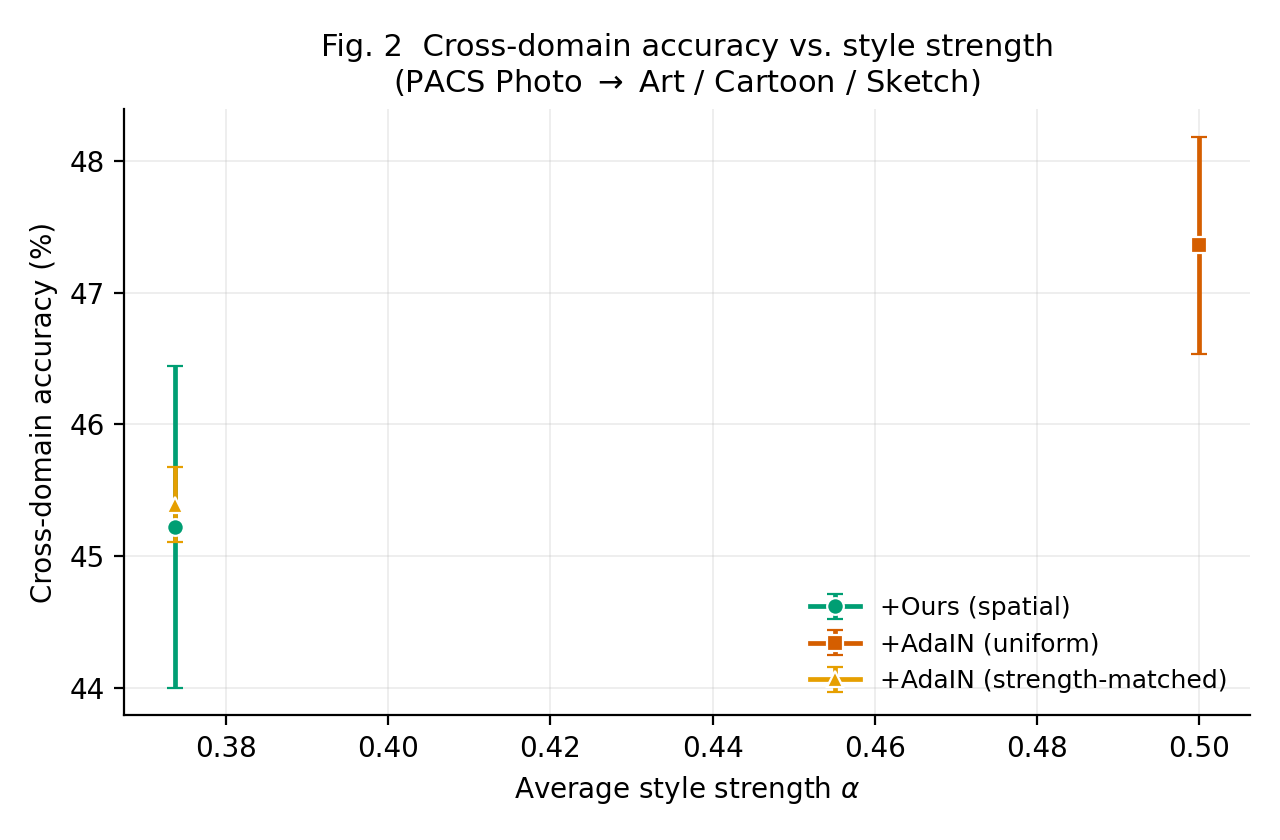
\includegraphics[width=\columnwidth]{../figures/strength_curve.png}
\caption{Cross-domain accuracy against the average style strength. Each point
is one trained configuration; the three series are the spatial variant, the
uniform AdaIN variant, and the strength-matched uniform control. The
configurations that differ in the \emph{spatial distribution} of the
strength lie on the same curve as the ones that differ in the strength
itself.}
\label{fig:strength_curve}
\end{figure}

\begin{figure}[t]
\centering
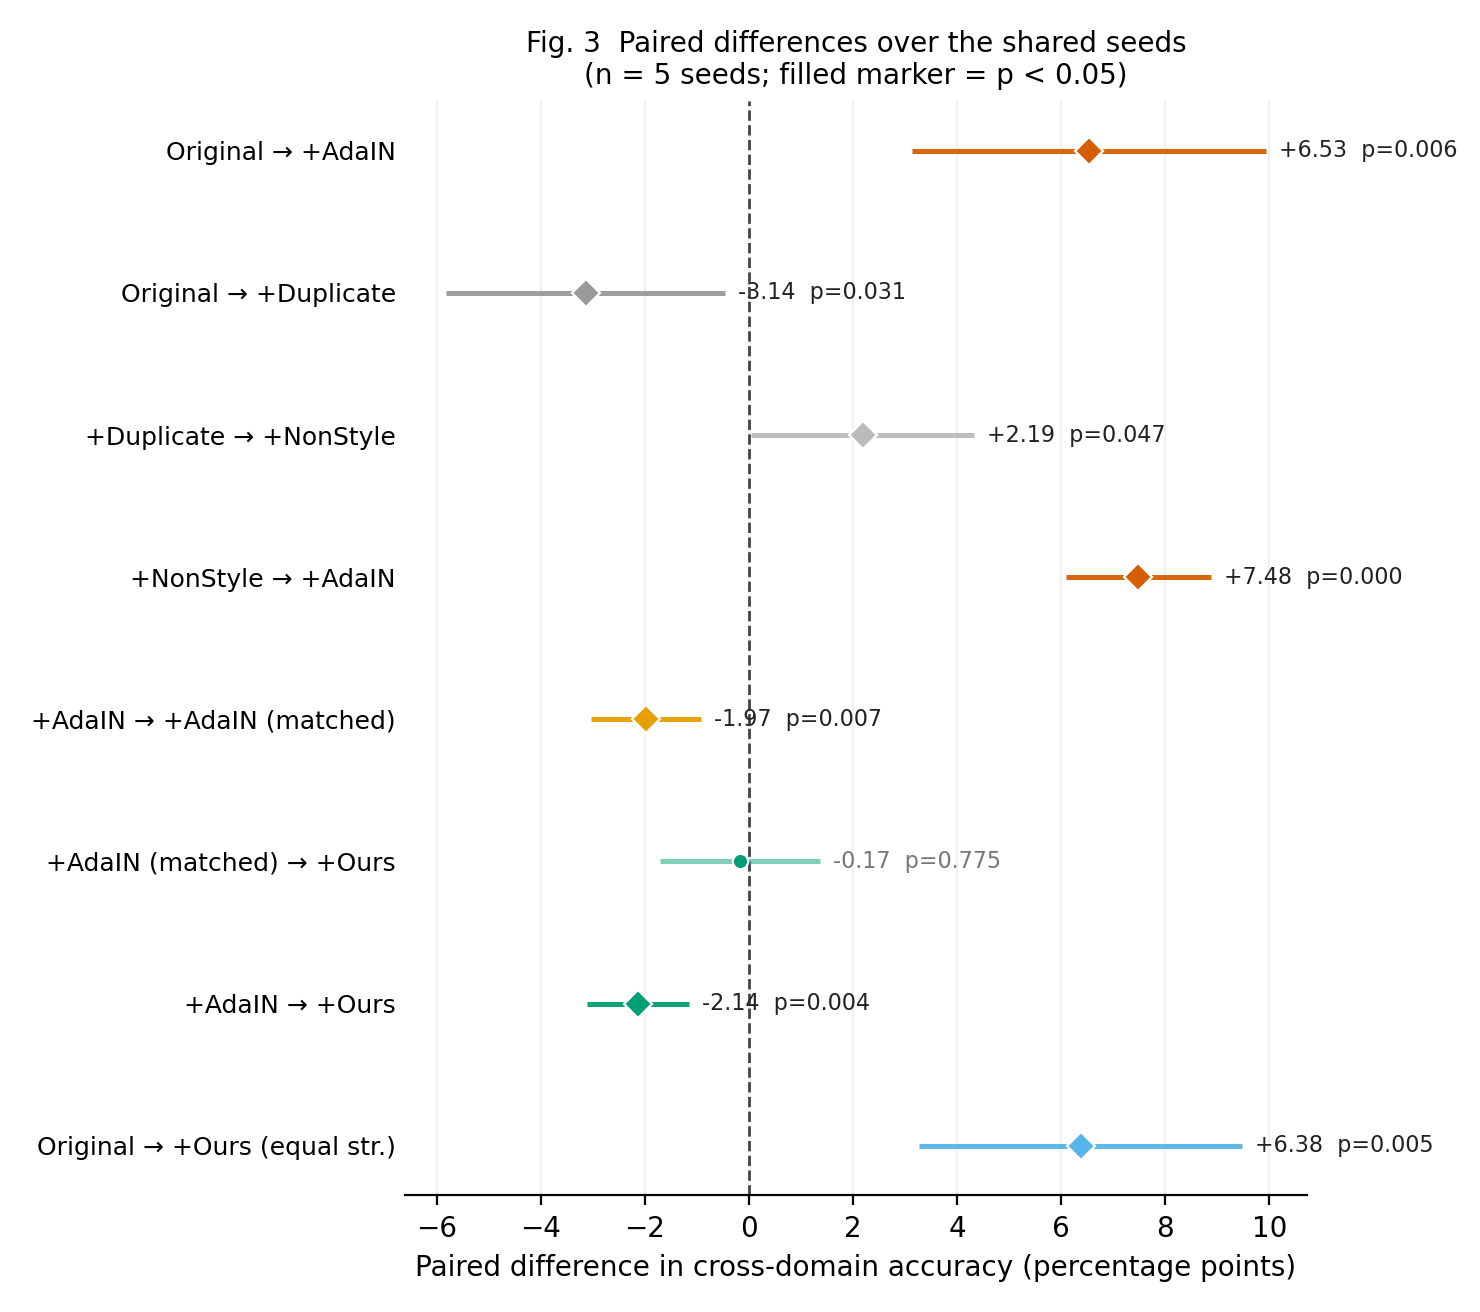
\includegraphics[width=\columnwidth]{../figures/forest_plot.png}
\caption{Paired differences between the experimental groups, with their 95\%
bootstrap confidence intervals. Every interval is computed over the shared
seeds of the two groups being compared.}
\label{fig:forest}
\end{figure}

\begin{figure}[t]
\centering
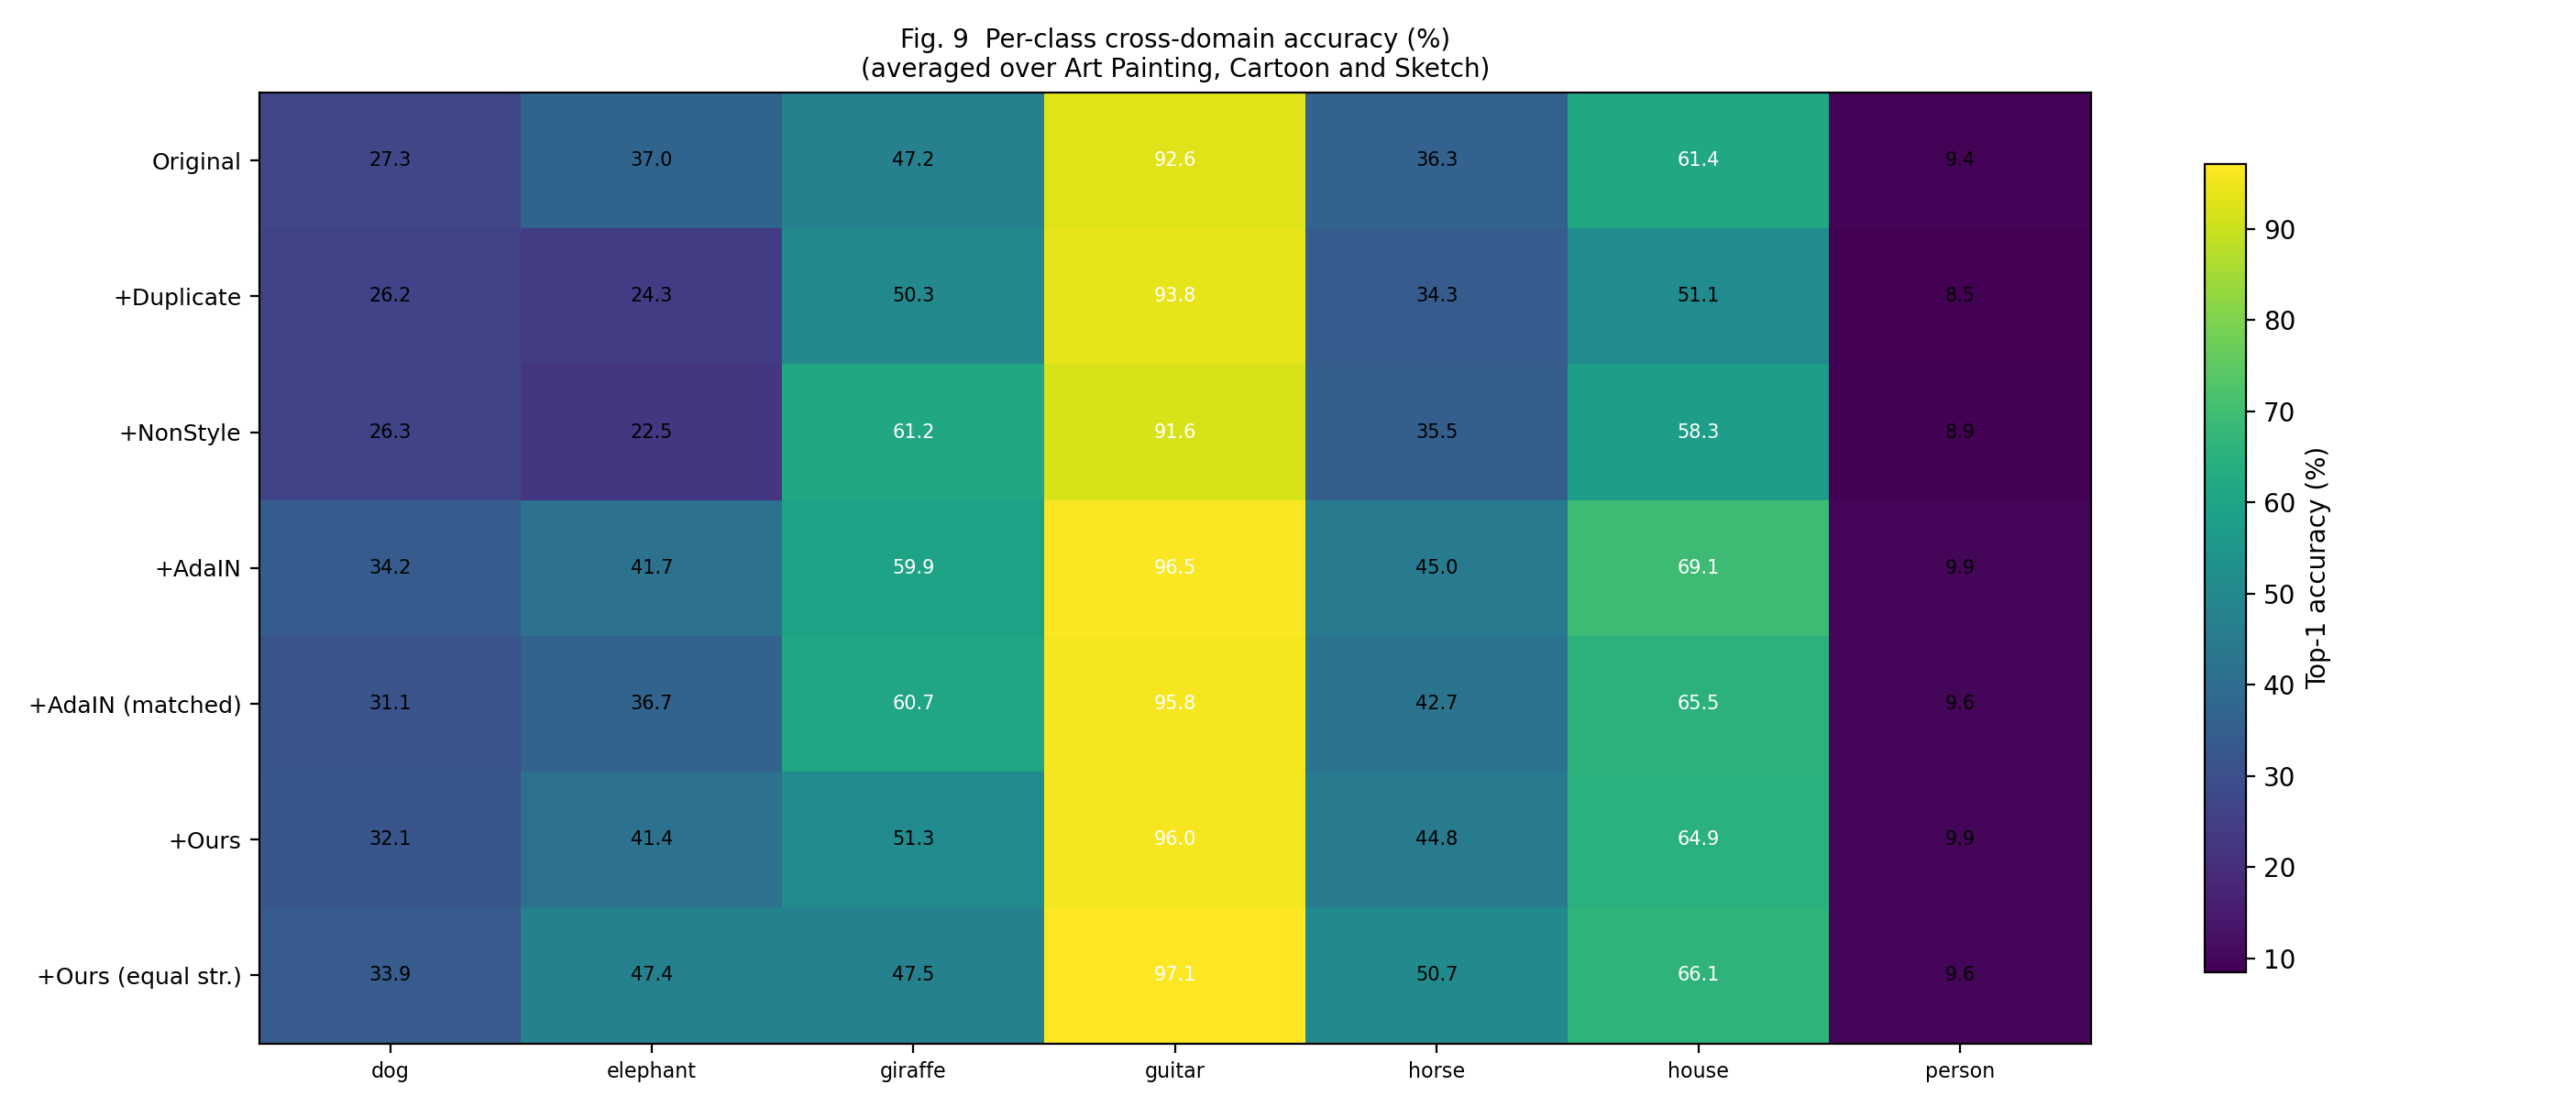
\includegraphics[width=\columnwidth]{../figures/per_class_heatmap.png}
\caption{Per-class cross-domain accuracy of the main groups. The gain over
the Original group is concentrated in the classes whose identity depends on
a shape rather than on a texture.}
\label{fig:per_class}
\end{figure}

%==================================================
\section{Conclusion and Future Work}
%==================================================

% Member 4 - final report, V Conclusion and Future Work
\section{Conclusion and Future Work}
\label{sec:conclusion}

We set out to find out what a style augmentation actually buys, and the answer turned out to be less than the method's premise suggests. Under a single-source Photo-only protocol on PACS, adding styled images to the training set improves cross-domain accuracy substantially, and the improvement survives the controls we designed to challenge it: doubling the number of training rows with byte-identical copies does not reproduce it, and neither does doubling them with non-stylistic transforms. The part of the gain that remains is attributable to the style itself.

The adaptive variant did not survive its control. A spatial strength map that applies less style where the content's structure is strong necessarily applies less style in total than a uniform mix at the same nominal strength, so a direct comparison confounds two factors. Once we hold the average strength fixed --- with a strength-matched uniform control and with a spatial map recalibrated to the same mean --- the two methods are indistinguishable in accuracy, and the per-image edge-retention analysis shows that the modulation does not preserve structure more selectively than the uniform alternative either. The mechanism the method was designed around is not observable in the images, and it is not observable in the classification result.

We draw three conclusions. First, style augmentation is a real and useful intervention on PACS, and it is worth the extra generation cost. Second, its benefit should be attributed to the amount of style applied rather than to the spatial structure preservation that motivated one line of work on it; the dose--response curve over $\alpha$ makes this explicit. Third, and most usefully for the field, the controls that make these attributions possible are cheap: a duplicate control and a strength-matched control are one extra generator and one extra training run each, and without them a headline gain can be reported for the wrong reason.

Several directions remain open. The soft Sobel response that drives the spatial map cannot tell a class-relevant contour from a texture edge; a semantic segmentation model would give a more selective map, and whether a selective map helps is the natural next experiment. The evidence here comes from one architecture and one dataset, so a ResNet-50 and a second domain-generalization benchmark would test how far the conclusion travels. And the third row of the decomposition remains an upper bound: separating "styling against a generic transform" from "one family of transforms against a random one" would need a finer set of controls. We are releasing the run artefacts and the checking machinery so that the decomposition can be re-run and extended.


%==================================================
\bibliographystyle{IEEEtran}
\bibliography{references}
%==================================================

\end{document}
